%%%%%%%%%%%%%%%%%%%%%%%%%%%%%%%%%%%%%%%%%
% 模板資訊:
% 模板名稱:Ernie's Beamer
% 版本:1.0 (2023.03.24)
% 修改者:莊程翔 Ernie Cheng-Xiang Zhuang
% 編譯器:XeLaTeX
%
% 原始模板的資訊:
% 模板名稱:Beamer Presentation
% 作者:Vel (vel@latextemplates.com)
% 編譯器:XeLaTeX
% 授權:CC BY-NC-SA 4.0 (https://creativecommons.org/licenses/by-nc-sa/4.0/)
% 下載連結:https://www.LaTeXTemplates.com
%
% 製作本模板之目的:
% 由於,LaTeX 對初學者來說不太友善,因此我針對 Vel 製作的模板做了大幅度的修改及附上清楚明瞭的註解,同時添加了許多常用且好用的封包,並增添了許多常用的客製化設定指令,以便 LaTeX 初學者能夠輕鬆地完成專業的學術簡報。
% 如果您有任何問題,可以透過以下兩種方式聯繫我:
% 1. 網站:https://www.ernie-zhuang.com/contact
% 2. Email:erniezhuang1127@gmail.com
%%%%%%%%%%%%%%%%%%%%%%%%%%%%%%%%%%%%%%%%%

%----------------------------------------------------------------------------------------
%	封包與文檔配置
%----------------------------------------------------------------------------------------

% 設定字型為12pt (可換成:8pt、9pt、10pt、11pt (默認)、12pt、14pt、17pt 或 20pt)
% 設定顯示比例為16:9 (可換成:1610、149、54、43 (默認) 或 32)
% 若有設定動畫,且要輸出記得加上 handout,避免列印過多相似的頁面。
\documentclass[12pt, aspectratio=169]{beamer} 

%%%%%%%%%%%%%%%%%%%%%%%%%%%%%%%%%%%%%%%%%
% 模板資訊:
% 模板名稱:Ernie's Beamer
% 版本:1.0 (2023.03.24)
% 修改者:莊程翔 Ernie Cheng-Xiang Zhuang
% 編譯器:XeLaTeX
%
% 原始模板的資訊:
% 模板名稱:Beamer Presentation
% 作者:Vel (vel@latextemplates.com)
% 編譯器:XeLaTeX
% 授權:CC BY-NC-SA 4.0 (https://creativecommons.org/licenses/by-nc-sa/4.0/)
% 下載連結:https://www.LaTeXTemplates.com
%
% 製作本模板之目的:
% 由於,LaTeX 對初學者來說不太友善,因此我針對 Vel 製作的模板做了大幅度的修改及附上清楚明瞭的註解,同時添加了許多常用且好用的封包,並增添了許多常用的客製化設定指令,以便 LaTeX 初學者能夠輕鬆地完成專業的學術簡報。
% 如果您有任何問題,可以透過以下兩種方式聯繫我:
% 1. 網站:https://www.ernie-zhuang.com/contact
% 2. Email:erniezhuang1127@gmail.com
%%%%%%%%%%%%%%%%%%%%%%%%%%%%%%%%%%%%%%%%%

%----------------------------------------------------------------------------------------
%	封包與文檔配置
%----------------------------------------------------------------------------------------

% 自訂字體的封包
\usepackage{fontspec} 

%% 設定中文字體
\usepackage{xeCJK}
\setCJKmainfont[AutoFakeBold=3.5 , AutoFakeSlant=0.2, Path = fonts/]{cwTeX_圓體.ttf}
\XeTeXlinebreaklocale "zh"
\XeTeXlinebreakskip = 0pt plus 1pt

%% 設定英文字體
\usefonttheme{serif} % 使用 serif 字體

% 自訂字體顏色的封包
\usepackage{color} 

%% 自訂顏色
\definecolor{NTHU_Purple}{RGB}{126,35,138}
\definecolor{Default_Blue}{RGB}{52,51,171}

% 數學工具及符號
\usepackage{mathtools, amsmath, amsfonts, amsthm, latexsym} 

% 分別將數學符號間的間隔加大及加粗
\usepackage{newtxtext,newtxmath}

% 圖表自動編號的封包
\usepackage[justification=centering]{caption} 
\usepackage[justification=centering, format=hang]{subcaption}

%% 設定自動編號
\setbeamertemplate{caption}[numbered]

%% 設定圖表編號及標籤的字體大小及字形
\captionsetup[figure]{font=small, labelfont=md}
\captionsetup[table]{font=small, labelfont=md}

% 導入圖形與表格的封包
\usepackage{graphicx}  % \scalebox{} 可用於將過大的表格縮小
\usepackage{booktabs}

% 排列多個子圖形的封包
\usepackage{subfigure} 

% 允許表格的一格能多列呈現的封包
\usepackage{multirow} 

% 可指定表格排版的封包
\usepackage{array}

% 序列標號
\usepackage{enumerate} 

% 繪圖封包 (用於添加浮水印)
\usepackage{tikz}

% 引注參考資料
\usepackage{natbib}

% 註釋掉大部分的封包
\usepackage{comment}

% 設定中文的標籤
\renewcommand{\figurename}{圖} 
\renewcommand{\tablename}{表} 

%----------------------------------------------------------------------------------------
%	排版形式 (擇一,不選等同選擇默認的排版形式)
%----------------------------------------------------------------------------------------

\mode<presentation>{
%\usetheme{default}
%\usetheme{AnnArbor}
%\usetheme{Antibes}
%\usetheme{Bergen}
%\usetheme{Berkeley}
%\usetheme{Berlin}
%\usetheme{Boadilla}
%\usetheme{CambridgeUS}
%\usetheme{Copenhagen}
%\usetheme{Darmstadt}
%\usetheme{Dresden}
%\usetheme{Frankfurt}
%\usetheme{Goettingen}
%\usetheme{Hannover}
%\usetheme{Ilmenau}
%\usetheme{JuanLesPins}
%\usetheme{Luebeck}
\usetheme{Madrid}
%\usetheme{Malmoe}
%\usetheme{Marburg}
%\usetheme{Montpellier}
%\usetheme{PaloAlto}
%\usetheme{Pittsburgh}
%\usetheme{Rochester}
%\usetheme{Singapore}
%\usetheme{Szeged}
%\usetheme{Warsaw}

%----------------------------------------------------------------------------------------
%	外框形式 (擇一,不選等同選擇默認的外框形式)
%----------------------------------------------------------------------------------------

%\useoutertheme{default}
%\useoutertheme{infolines}
%\useoutertheme{miniframes}
\useoutertheme{smoothbars}
%\useoutertheme{sidebar}
%\useoutertheme{split}
%\useoutertheme{shadow}
%\useoutertheme{tree}
%\useoutertheme{smoothtree}

%----------------------------------------------------------------------------------------
%	外框的自訂義調整 
%----------------------------------------------------------------------------------------

% 外框上緣的字 (fg) 為黑色,背景 (bg) 為白色。
%\setbeamercolor{section in head/foot}{fg=black, bg=white} 

% 外框上緣顯示的章節(section)頁數標籤是否關閉
%\setbeamertemplate{mini frames}{}  

% 調整外框形式的字體大小
\setbeamerfont{headline}{size=\scriptsize}
\setbeamerfont{footline}{size=\scriptsize}

% 取消右下方的跳轉工具列
\setbeamertemplate{navigation symbols}{} 

%% 自定義1:外框下緣僅出現名字及頁碼
%\setbeamertemplate{footline} 
%{\leavevmode%
%\hbox{%
%\begin{beamercolorbox}[wd=0.5\paperwidth,ht=3ex,dp=1ex,leftskip=3ex]%
%{author in head/foot}%
%{\scriptsize\textbf{\insertshortauthor}}%
%\end{beamercolorbox}%
%\begin{beamercolorbox}[wd=0.5\paperwidth,ht=3ex,dp=1ex,right]%
%{author in head/foot}%
%\scriptsize \textbf{{\insertframenumber{} / \inserttotalframenumber\hspace*{2ex}}} %頁碼控制選項
%\end{beamercolorbox}%
%}}

%% 自定義2:清除外框下緣但僅出頁碼
%\setbeamertemplate{footline}[page number] 

%% 自定義3:清除外框下緣
%\setbeamertemplate{footline}[] 

%----------------------------------------------------------------------------------------
%	顏色主題 (擇一,不選等同選擇默認的顏色主題)
%----------------------------------------------------------------------------------------

\usecolortheme{default}
%\usecolortheme{albatross}
%\usecolortheme{beaver}
%\usecolortheme{beetle}
%\usecolortheme{crane}
%\usecolortheme{dolphin}
%\usecolortheme{dove}
%\usecolortheme{fly}
%\usecolortheme{lily}
%\usecolortheme{orchid}
%\usecolortheme{rose}
%\usecolortheme{seagull}
%\usecolortheme{seahorse}
%\usecolortheme{whale}
%\usecolortheme{wolverine}

%----------------------------------------------------------------------------------------
%	顏色主題的自訂義調整 
%----------------------------------------------------------------------------------------

% 全文的主題色 (可以特別針對報告對象或機構的代表色調整!)
\setbeamercolor{structure}{fg=NTHU_Purple} 

% 封面頁中標題區塊的底色及字體顏色
%\setbeamercolor{title}{bg=green, fg=black} 

% 各頁標題區塊的底色及字體顏色
%\setbeamercolor{frametitle}{bg=green,fg=black} 

% 全文的內文顏色
%\setbeamercolor{normal text}{fg=orange}

% 數學區塊的標題顏色 
%\setbeamercolor{block title}{bg=blue,fg=yellow} 

% 數學區塊的內文顏色 
%\setbeamercolor{block body}{bg=green,fg=red} 

% 警示文字的顏色
\setbeamercolor{alerted text}{fg=red} 

%----------------------------------------------------------------------------------------
%	enumerate 及 item 的形狀
%----------------------------------------------------------------------------------------

\useinnertheme{rounded} % 圓球 (3D)
%\useinnertheme{circles} % 圓形 (2D)
%\useinnertheme{rectangles} % 方形
%\useinnertheme{inmargin} % 插入邊沿

%----------------------------------------------------------------------------------------
%	自訂 item 的顏色
%----------------------------------------------------------------------------------------

%\setbeamercolor{item projected}{bg=red}

%----------------------------------------------------------------------------------------
%	個人化的設置及細節調整
%----------------------------------------------------------------------------------------

% 設定頁面邊界
\setbeamersize{text margin left=0.8cm, text margin right=0.8cm}
\special{papersize=\the\paperwidth,\the\paperheight}
\providecommand{\tabularnewline}{\\}
}

%----------------------------------------------------------------------------------------
%	個人化的背景調控
%----------------------------------------------------------------------------------------

% 背景照片設置
%\setbeamertemplate{background}{
\includegraphics[height=\paperheight]{Fig/Background.png}}

% 浮水印設定
\usebackgroundtemplate{%
	\tikz[overlay, remember picture] % 讓 logo 能每頁都顯示
	\node[opacity=0.3, below=-1.25cm, at=(current page.center)] % 調整透明度 (opacity) 及浮水印的位置
	{
\includegraphics[scale = 0.14]{Fig/nthulogo.png}}; % 載入 logo 及調整大小
	}
 % 載入封包與文檔配置

\begin{document}

%----------------------------------------------------------------------------------------
%	簡報資訊
%----------------------------------------------------------------------------------------

% [] 內為顯示於外框中的文字,{} 則是封面上的文字。

% 簡報名稱
\title[\LaTeX{}  Beamer 如何做?]{\Huge{\textbf{\LaTeX{} Beamer 如何做?}}} 

% 簡報子名稱
\subtitle{各種可能所需的頁面模板} 

% 作者
\author[Ernie Cheng-Xiang Zhuang]{% 
莊程翔  \thanks{國立清華大學經濟學系} \and%
Ernie Cheng-Xiang Zhuang \thanks{National Tsing Hua University}
}

% 機構
\institute[NTHU]{\normalsize 國立清華大學 National Tsing Hua University} 

% 日期
\date[\today]{\today}

%----------------------------------------------------------------------------------------
%	封面頁
%----------------------------------------------------------------------------------------

\begin{frame}
	\titlepage % 將上方資訊輸出成封面頁
\end{frame}

%----------------------------------------------------------------------------------------
%	目錄
%----------------------------------------------------------------------------------------

\begin{frame}{\textbf{目錄}}
	\tableofcontents % 將所有節及子節的內容輸出成表
\end{frame}

%----------------------------------------------------------------------------------------
%	(動畫)字會若隱若現的顯示
%----------------------------------------------------------------------------------------

% (動畫)字會若隱若現的顯示
\beamersetuncovermixins{\opaqueness<1->{45}}{\opaqueness<1->{95}} 

%----------------------------------------------------------------------------------------
%	文字處裡
%----------------------------------------------------------------------------------------

\section{文字處裡}

%----------------------------------------------------------------------------------------

\linespread{1}  % 此行以後,皆為1倍行高
\begin{frame}{\textbf{文字處裡}}
\linespread{1.5} % 此行以後,皆為1.5倍行高

	研究表明,
	漢字的序順並不定一能影閱響讀,
	比如當你看這句話後,
	才發這現裡的字全是都亂的。
	
	% 垂直距離的空格 (另外有\medskip, \smallskip, \vspace{?em})
	 \bigskip 
	 
	 % 動畫出現至此的指令
	\pause 
	
	% alert 是讓字變紅色, \textbf 是讓字變粗體,\textit 則是變斜體。
	 \alert{Econometrics} is a \textbf{statistical} method used to \textit{estimate} the economic relationship,
	 test economic theories, and evaluate the effects of government or business policies.
	 
	 \pause
	
	\bigskip 

	% 引用名言
	\begin{quote}
		Pure mathematics is, in its way, the poetry of logical ideas.\\
		(純粹數學,就其本質而言,是邏輯思想的詩篇。)\\
		--- Albert Einstein (愛因斯坦)
	\end{quote}
	
\end{frame}

%----------------------------------------------------------------------------------------
%	項目編號及數字編號
%----------------------------------------------------------------------------------------

\section{項目編號及數字編號}

%----------------------------------------------------------------------------------------

% [<+>] 會自動以動畫呈現,就不用一直輸入 \pause。
\linespread{1} 
\begin{frame}[<+>]{\textbf{項目編號及序列編號}}
\linespread{1.5} 

	\begin{itemize}[] % 封包 itemize 的 item
		\item 這是封包 itemize 的 item
		\begin{enumerate}[] % 封包 enumerate 的 item,[] 中不輸入東西。
			\item 這是封包 enumerate 的 item
			\item 比較一下兩者:
				\begin{enumerate}[1] % 封包 enumerate 的 item,[] 中輸入 1。
					\item 封包 itemize 的 item 明顯較小
					\item 封包 enumerate 的 item 則較大
					\item 另外,可觀察到文字越往內層會逐漸稍微縮小。
				\end{enumerate}
		\end{enumerate}
	\end{itemize}
	
\end{frame}

%----------------------------------------------------------------------------------------
%	數學的區塊文字
%----------------------------------------------------------------------------------------

\section{數學}

%----------------------------------------------------------------------------------------

\linespread{1} 
\begin{frame}{\textbf{數學的區塊文字}}
\linespread{1.5}

	\begin{block}{\textbf{定義}} 
		一個二次可微分的實數函數$f\left(x\right)$稱為一個凸函數(convex function),
		若$f^{\,\prime\prime}\!\left(x\right)\ge0$對所有$x$;
		同理若$f^{\,\prime\prime}\!\left(x\right)\le0$對所有$x$,
		則稱為凹函數(concave function)。
	\end{block}
	
	\begin{block}{\textbf{證明}} 
		若要在證明的方塊後加入實心正方形,
		可以輸入$\backslash$hfill\$$\backslash$blacksquare\$。
		\hfill$\blacksquare$
	\end{block}
	
\end{frame}

%----------------------------------------------------------------------------------------

\linespread{1} 
\begin{frame}{\textbf{數學的區塊文字 (續)}}
\linespread{1.5} 

	\begin{alertblock}{\textbf{引裡}}
		我的書寫空間不足了,
		您可依前面的架構自行更改。
	\end{alertblock}
	\label{連結的文字} % 為 \hyperlink{連結的文字} 到達的地方
	
	\begin{example}
		可以發現三個環境指令的不同之處:
		\begin{itemize}
			\item block 跟背景色一致
			\item alertblock 是紅色的
			\item example 則是綠色的
		\end{itemize}
	\end{example}
	
\end{frame}

%----------------------------------------------------------------------------------------

\linespread{1} 
\begin{frame}[<+>]{\textbf{數學方程式}}
\linespread{1.5} 
	
	% 數學式中,我們會適時加入符號來增減空隙。
	%% \, 增加 1.5pt 
	%% \! 減少 1.5pt
	%% \: 增加 3pt
	%% \; 增加 5pt
	\begin{align}\label{reg}
		\ln\left[\frac{Prob.\left(Y=b|X\right)}{Prob.\left(Y=0|X\right)}\right]
			=\beta_0+\sum_{j=1}^k \beta_{i,j}\,X_{i,j,b|Y=0}+\varepsilon_{i,b|Y=0}
	\end{align}

	\begin{align}\label{var}
		\left(n-1\right)\!S^{\,2} & =  \sum_{i=1}^{n}\left(x_{i}-\widebar{X}\right)^{2} 
			 =  \sum_{i=1}^{n}x_i^{\,2}-n\widebar{X}^{\,2} \notag \\
		\Rightarrow \sum_{i=1}^{n} x_i^{\,2} & =  \left(n-1\right)\!S^{\,2}+\underbrace{n \widebar{X}^{\,2}}_{\text{校正項}}
	\end{align}

\end{frame}

%----------------------------------------------------------------------------------------
%	插入單頁圖片
%----------------------------------------------------------------------------------------

\section{圖表製作}

%----------------------------------------------------------------------------------------

\subsection{圖片}

%----------------------------------------------------------------------------------------

\linespread{1}  
\begin{frame}{\textbf{插入圖片}}
\linespread{1.5}
	
	\begin{figure}
		\centering % 置中
		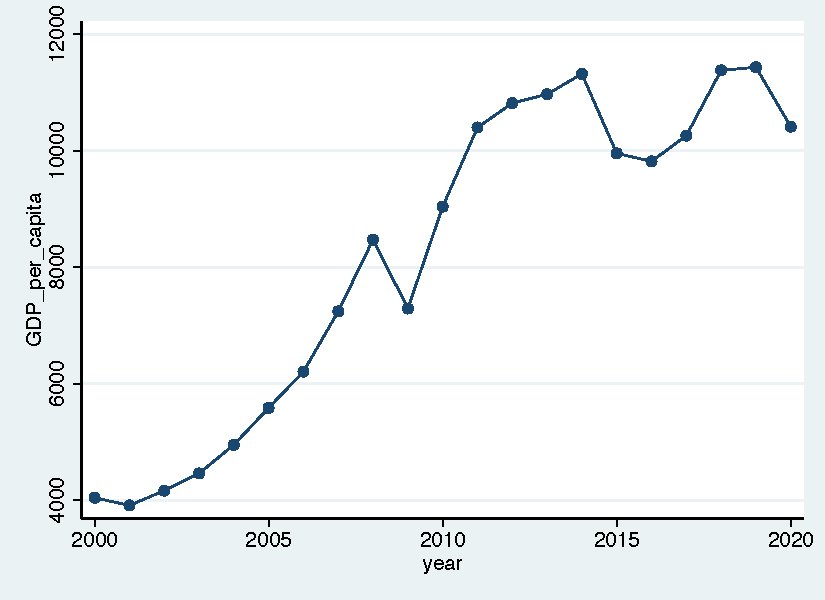
\includegraphics[scale=0.45]{Fig/GDP_per_capita.pdf}\\ % 導入圖片並調整大小
		\hspace{-9em}\scriptsize{資料來源:Worldbank。}\\ % 調整位置並輸入資料來源
		\vspace{-0.5em} % 縮減垂直距離
		\caption{馬來西亞的GDP per capita (current US\$)} % 圖片名稱
		\label{GDP_per_capita} % 建立圖標籤
	\end{figure}
	
\end{frame}

%----------------------------------------------------------------------------------------
%	加入單頁表格
%----------------------------------------------------------------------------------------

\subsection{表格}

%----------------------------------------------------------------------------------------

\linespread{1}  
\begin{frame}{\textbf{插入表格}}
\linespread{1.5} 

	\begin{table}[htbp]
		\centering % 置中
		\caption{公立、私立大學的就學貸款統計差異(108 學年度)} % 表名
		\extrarowheight=2pt % 額外增加每列的寬度
		\label{loan} % 建立表標籤
		\scalebox{0.9}{ % 將表縮小,不要縮小可以調成 1。
		\begin{tabular}{p{5cm} p{3cm}<{\centering} p{3cm}<{\raggedleft}} % 控制欄寬,及文字對齊方式。
			\toprule
			\midrule
 			& 公立大學 & 私立大學\\
			\midrule
			貸款金額 & 3,121,271,506 & 16,098,465,719 \\
			貸款學生人數 & 55,715 & 187,076 \\
			學生人數 & 439,073 & 774,099 \\
			人均貸款金額 & 56,022 & 86,053 \\
			貸款學生人數/學生人數 & 12.69\% & 24.17\% \\
			\midrule
			\bottomrule
		\end{tabular}
		}
		\par\smallskip
		\hspace{2em}\parbox{0.8\textwidth}{\scriptsize % 調整資料來源及表註的位置、字體大小及文字寬度。
		資料來源:\href{https://helpdreams.moe.edu.tw/hd/upload/20201211_1.pdf}{圓夢助學網}。\par
		註:\parbox[t]{0.6\textwidth}{\scriptsize % 記得稍微小於前兩行的 \textwidth
		可在此處增加表格備註。
		}
		}
	\end{table}
	
\end{frame}

%----------------------------------------------------------------------------------------

\linespread{1} 
\begin{frame}{\textbf{插入表格 (續)}}
\linespread{1.5} 

	\begin{table}[htbp]
		\centering 
		\caption{CareerCast 近五年五大最佳職業} 
		\extrarowheight=2pt 
		\label{CareerCast} 
		\scalebox{0.8}{ 
		\begin{tabular}{@{}crrrr@{}} % @{} 表示表的左右兩端之文字沿著表邊緣;lcr 可分別讓文字對齊左邊、中間、右邊,且寬度自動偵測。
			\toprule
			\midrule
			 排名 & 2021 &  2019 & 2018 & 2017\\
			\midrule
			1 & { 資料科學家} & \textbf{資料科學家}  &  遺傳諮詢師 & \textbf{統計學家} \\
			2 & 遺傳諮詢師 & \textbf{統計學家} & \textbf{數學家}  & 醫療服務經理 \\
			3 & \textbf{統計學家} & 大學教授  & 大學教授 & \textbf{作業研究分析師}\\
			4 & 醫療服務經理 & 職能治療師  & 職能治療師 & \textbf{資訊安全分析師} \\
			5 & \textbf{數學家} & 遺傳諮詢師 & \textbf{統計學家} & \textbf{資料科學家} \\
			\midrule
			\bottomrule
		\end{tabular}
		}
		\par\smallskip
		\hspace{0.5em}\parbox{0.6\textwidth}{\scriptsize
		資料來源:CareerCast, 取自:\url{https://www.careercast.com}。\par
		註:\parbox[t]{0.5\textwidth}{\scriptsize
		1、2020 年 CareerCast 沒有公布年度十大最佳職業。\\
		 2、粗體為理工科 (STEM) 相關的職業。
		}
		}
	\end{table}

\end{frame}

%----------------------------------------------------------------------------------------
%	兩欄圖文 (也可變成三欄、四欄⋯)
%----------------------------------------------------------------------------------------

\section{兩欄圖文}

%----------------------------------------------------------------------------------------

\linespread{1}  
\begin{frame}{\textbf{兩欄圖文 (或多欄)}}
\linespread{1.5} 

	\begin{columns}[c] % 開啟多欄的環境
		\column{0.67\textwidth} % 設定欄寬
			\begin{enumerate}[]
				\item 我們在內文中要提及前面的圖、表或方程式時,應該這樣引注:
				\begin{enumerate}[]
					\item 「圖 $\backslash$ref\{label 內的名字\}」,
						即可出現圖 \ref{GDP_per_capita} 和圖 \ref{LaTeX}。
					\item 「表 $\backslash$ref\{label 內的名字\}」,
						即可出現表 \ref{loan} 與表 \ref{CareerCast}。
					\item 「式 ($\backslash$ref\{label 內的名字\})」,
						即可出現式 (\ref{reg}) 和式 (\ref{var})。
				\end{enumerate}
				\item 引注的好處是簡報有所更動時,不用一直手動調整編號。
			\end{enumerate}

		\column{0.33\textwidth} % 設定欄寬
			\begin{figure}
				
\includegraphics[scale=0.045]{Fig/LaTeX.png}\\
				\scriptsize{資料來源:
				\href{https://en.wikipedia.org/wiki/LaTeX}{維基百科}。}\\
				\caption{\LaTeX}
				\label{LaTeX} 
			\end{figure}
	\end{columns}
\end{frame}


%----------------------------------------------------------------------------------------
%	其他
%----------------------------------------------------------------------------------------

\begin{frame}

	建立無標題頁面,並且展示超連結按鈕。
	
	\bigskip
	
	\hyperlink{連結的文字}{\beamergotobutton{連結}} % 超連結按鈕
	
\end{frame}

%----------------------------------------------------------------------------------------
%	參考資料
%----------------------------------------------------------------------------------------

\section{參考資料}

%----------------------------------------------------------------------------------------

\linespread{1} 
\begin{frame}{\textbf{引用參考資料的方法}}
\linespread{1.5}

	引用參考資料文章的方法:
	
	\begin{enumerate}[1]
		\item 將文獻作者當作主詞時使用時:\textbackslash citet\{給定的標籤\}。
		\item 行文末端作為補充說明時:\textbackslash citep\{給定的標籤\}。
	\end{enumerate}
	
	\bigskip
	
	以本文為例:
	
	\begin{enumerate}[1]
		\item \citet{Non-CES} 與 \citet{期刊評比}
		\item \citep{Non-CES} 與 \citep{期刊評比}
	\end{enumerate}
	
\end{frame}

%----------------------------------------------------------------------------------------

\linespread{1} 
\begin{frame}{\textbf{參考資料}}
\linespread{1.5} 

\footnotesize

\begin{thebibliography}{99} 

	\bibitem[K. Matsuyama (2022)]{Non-CES} % 引注時顯示的名稱
		K. Matsuyama (2022). % 作者 (年份)
		\newblock Non-CES Aggregators: A Guided Tour, % 文章名稱
		\newblock \emph{Annual Review of Economics}, 15, forthcoming. % 期刊名稱、章節及頁碼。

	\bibitem[林明仁、林常青、張俊仁、曹添旺與楊浩彥 (2019)]{期刊評比} 
		林明仁、林常青、張俊仁、曹添旺與楊浩彥 (2019)。 
		\newblock 經濟學門學術期刊評比更新:2019年,
		\newblock \emph{經濟論文叢刊},47(4),503--542。
		
\end{thebibliography}

\end{frame}

%----------------------------------------------------------------------------------------
%	結束頁
%----------------------------------------------------------------------------------------

\section*{結束頁}

%----------------------------------------------------------------------------------------

\begin{frame}[plain] % 產生無外框的頁面

	\begin{center}
		{\Huge The End}
		
		\bigskip\bigskip 
		
		{\LARGE Questions? Comments?}
	\end{center}
	
\end{frame}

%----------------------------------------------------------------------------------------

\end{document} 